\scanpage{467}
\mspage{236}

operates on $X_g$.

One should now, along these lines:

1) Make explicit the outer action of this $\frac12$ direct product on the fundamental group $\pi_g$, \unsure{with} very special attention to the action of the group $(\mathbb Z/2\mathbb Z)^3\subset\mathbb D_{2g}^{\sim}$ which stabilizes one of the cylinders $T_j$ --- which in Euclidean space of dimension 3 is interpreted as the group of \unsure{changes} of sign relative \unsure{to the|a} corresponding orthonormal system of axes.

2) Extend the action \inserted{on $\pi_g$} of the (more or less) ``special'' Teichmüller group of each of the $T_j$, to the action of an analogous group of a larger set obtained by adding to it a ``strip'' \inserted{$L$} (whence a torus with 1 hole, and its special Teichmüller group, which \unsure{come in} naturally$^*$) \unsure{or even|see} the still larger set obtained by also putting in the antipodal strip $L'$ (this set presents itself as a cylinder $(L\cup L')$, or ``culvert'', in which one would have put a tube $(T_j)$ crosswise, and has the topological structure of a torus with two holes.

\figure{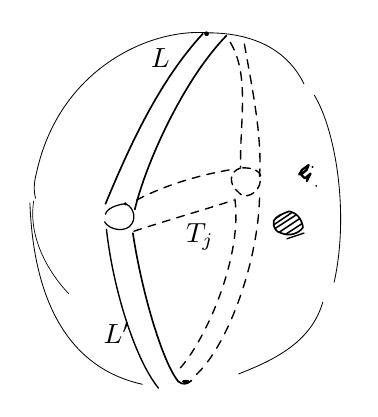
\begin{tikzpicture}[x=.12mm,y=-.12mm,line cap=round,line join=round]
\draw[line width=.3pt] (194,39) .. controls (133,34) and (37,77) .. (13,187) .. controls (10,198) and (10,207) .. (12,214);
\draw[line width=.3pt] (194,39) .. controls (244,39) and (279,58) .. (296,93);
\draw[line width=.3pt] (307,105) .. controls (330,143) and (344,231) .. (328,303);
\draw[line width=.3pt] (316,324) .. controls (304,365) and (268,384) .. (227,400);
\draw[line width=.3pt] (6,219) .. controls (9,303) and (35,391) .. (125,411);
\draw[line width=.25pt] (10,217) .. controls (4,255) and (25,292) .. (47,315);
\draw[line width=.6pt] (189,40) .. controls (142,91) and (111,160) .. (86,220);
\draw[line width=.6pt] (214,42) .. controls (169,88) and (129,176) .. (117,226);
\draw[line width=.5pt] (87,247) .. controls (94,310) and (117,384) .. (142,415);
\draw[line width=.6pt] (115,251) .. controls (124,312) and (146,387) .. (163,408) .. controls (168,412) and (172,411) .. (177,407);
\draw[line width=.45pt] (86,231) .. controls (87,225) and (98,221) .. (106,220) .. controls (114,221) and (119,233) .. (114,241) .. controls (108,251) and (90,248) .. (85,239);
\draw[line width=.5pt,dash pattern=on 1.1mm off .9mm] (218,49) .. controls (239,84) and (228,133) .. (229,181);
\draw[line width=.5pt,dash pattern=on 1.1mm off .9mm] (233,51) .. controls (241,96) and (252,149) .. (249,191);
\draw[line width=.5pt,dash pattern=on 1mm off .7mm] (229,182) .. controls (216,186) and (217,200) .. (226,207) .. controls (233,217) and (249,209) .. (250,195) .. controls (253,186) and (242,181) .. (229,182);
\draw[line width=.5pt,dash pattern=on 1mm off 1mm] (223,215) .. controls (231,278) and (191,366) .. (164,395);
\draw[line width=.5pt,dash pattern=on 1.1mm off 1mm] (249,214) .. controls (247,288) and (211,380) .. (177,405);
\draw[line width=.5pt,dash pattern=on 1mm off .9mm] (119,216) .. controls (155,197) and (197,187) .. (224,183);
\draw[line width=.5pt,dash pattern=on 1mm off .9mm] (116,249) .. controls (156,236) and (198,224) .. (222,216);
\fill (193,40) circle[radius=.3mm];
\fill (171,408) ellipse[x radius=.48mm,y radius=.216mm];
\fill (107,220) circle[radius=.216mm];
\node[inner sep=0pt] at (144,66) {$L$};
\node[inner sep=0pt] at (98,357) {$L'$};
\node[inner sep=0pt] at (186,255) {$T_j$};
\draw[line width=.8pt] (291,189) -- (294,184) -- (301,179) -- (299,184) -- (293,189) -- (297,193) -- (303,188) -- (299,196);
\fill (305,181) circle[radius=.144mm];
\fill (309,201) circle[radius=.132mm];
\draw[line width=.6pt] (264,238) .. controls (266,233) and (275,230) .. (280,228) .. controls (288,229) and (294,236) .. (295,245) .. controls (291,251) and (281,255) .. (272,251) .. controls (266,250) and (263,244) .. (264,238);
\begin{scope}
\clip (264,238) .. controls (266,233) and (275,230) .. (280,228) .. controls (288,229) and (294,236) .. (295,245) .. controls (291,251) and (281,255) .. (272,251) .. controls (266,250) and (263,244) .. (264,238);
\draw[line width=.55pt] (258,241)--(283,224) (260,245)--(288,226) (261,249)--(292,229) (264,254)--(297,232) (271,256)--(300,237) (280,257)--(302,242);
\end{scope}
\draw[line width=.5pt] (278,257) -- (296,251);
\end{tikzpicture}}

\margin{$^*$ This is essentially an $\mathrm{SL}(2,\mathbb Z)$ --- rather a \unsure{remarkable} central extension of $\mathrm{SL}(2,\mathbb Z)$ by $\mathbb Z$, which \unsure{recalls} that of $\mathrm{SL}(2,\mathbb R)$ by $\mathbb Z$\ldots\ (universal covering of $\mathrm{SL}(2,\mathbb R)$)}

\figure{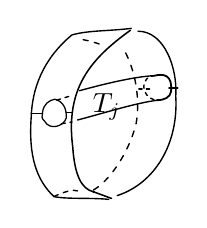
\begin{tikzpicture}[x=.12mm,y=-.12mm,line cap=round,line join=round]
\draw[line width=.5pt] (118,15) .. controls (94,18) and (72,17) .. (55,22) .. controls (24,48) and (13,79) .. (12,109) .. controls (9,151) and (18,176) .. (36,193) .. controls (49,196) and (75,194) .. (94,196);
\draw[line width=.5pt] (125,18) .. controls (153,18) and (167,57) .. (165,87) .. controls (168,137) and (143,179) .. (103,192);
\draw[line width=.55pt] (117,17) .. controls (74,48) and (48,79) .. (56,141) .. controls (58,170) and (65,185) .. (78,188) -- (97,195);
\draw[line width=.5pt,dash pattern=on .65mm off .8mm] (67,27) .. controls (74,28) and (82,31) .. (89,33);
\draw[line width=.5pt,dash pattern=on .75mm off .95mm] (112,41) .. controls (124,65) and (127,94) .. (123,116) .. controls (115,148) and (94,177) .. (78,186);
\draw[line width=.45pt] (24,104) .. controls (25,95) and (31,91) .. (37,90) .. controls (46,92) and (50,101) .. (49,110) .. controls (47,118) and (32,124) .. (26,113) .. controls (23,111) and (23,107) .. (24,104);
\draw[line width=.5pt] (12,105) -- (24,105) (49,104) -- (55,104);
\draw[line width=.5pt,dash pattern=on .5mm off .6mm] (39,91) -- (55,86) (44,116) -- (55,114);
\draw[line width=.5pt] (63,81) .. controls (85,75) and (120,66) .. (143,65);
\draw[line width=.5pt] (61,112) .. controls (88,105) and (122,94) .. (146,91);
\draw[line width=.65pt] (143,65) .. controls (159,61) and (161,72) .. (160,82) .. controls (159,88) and (153,91) .. (145,91);
\draw[line width=.5pt,dash pattern=on .45mm off .55mm] (143,65) .. controls (128,65) and (126,87) .. (144,91);
\draw[line width=.55pt,dash pattern=on .4mm off .55mm] (126,79)--(141,79);
\draw[line width=.7pt] (158,78)--(167,78);
\draw[line width=.5pt,dash pattern=on .6mm off .7mm] (36,193) .. controls (47,188) and (56,185) .. (61,187);
\fill (78,188) circle[radius=.18mm];
\node[inner sep=0pt] at (92,98) {$T_j$};
\end{tikzpicture}}

\margin{466}

\scanpage{468}

It is possible that it will be necessary to look closely at this last one, to study the relations among \inserted{the} elements of $\mathcal T_g$ coming from the preceding sets\ldots\ An amusing job will be to manage to write down the generators of the group $\pi_g$, and above all the famous relation, in a relative geometric arrangement of the ``handles'', which is a ``\unsure{mixed}'' arrangement --- and no longer \uline{nicely} in single file!

\deleted{I see \unsure{appearing}}

While waiting to get to the heart of the structure of the Teichmüller group in this way, I will already try to describe generators and relations for the interesting subgroup we have just written down, $\mathbb D_{2g}^{\sim}\cdot H$.
I will take the everlasting generators $\varepsilon_0,\varepsilon_1$ of $\mathbb D_{2g}$
\[
\varepsilon_0^2=\varepsilon_1^2=1,\qquad (\varepsilon_0\varepsilon_1)^{2g}=1
\]
and adjoin to them $\tau=\tau_g$, and \deleted{\illegible{1}} $\rho_0\tau=\tau'$
($\rho_0=\rho_{j_0}$, $j_0$ marked point of $I=J/\tau$)
satisfying
\[
\tau^2=\tau'^2=1,\qquad
\deleted{[\tau,\varepsilon_0]=\unsure{[\varepsilon_1,\tau]|[\tau,\varepsilon_1]}=}
\]
\[
(\tau\varepsilon_0)^2=(\tau\varepsilon_1)^2=1\quad
\deleted{\unsure{(\tau'\varepsilon_0)^2=(\tau'\varepsilon_1)^2}=1}
\]
\[
(\varepsilon_1\tau')^2=1
\qquad \varepsilon_1\ \text{commutes with}\ \tau'
\]

\margin{\uline{N.B.} $\varepsilon_0$ moves \unsure{the vertex} of the frame, $\varepsilon_1$ the edge and not the vertex, hence $\varepsilon_1(j_0)=j_0$}

\margin{\unsure{express} the commutation of $\tau$ \deleted{\illegible{1}} with $\varepsilon_0,\varepsilon_1$}

\margin{467}

\scanpage{469}
\mspage{237}

\[
((\varepsilon_0\varepsilon_1)^g\tau')^2=1
\]
\margin{(the involution $(\varepsilon_0\varepsilon_1)^g$ commutes with $\tau'$)}

unless I am mistaken, that gives a set of generators and relations for $\mathbb D_{2g}^{\sim}\cdot\mathcal H$ --- in summary $\varepsilon_0,\varepsilon_1,\tau,\tau'$
\[
\text{(52)}\quad
\left\{
\begin{array}{l}
\varepsilon_0^2=\varepsilon_1^2=\tau^2=\tau'^2=1\\
(\tau\varepsilon_0)^2=(\tau\varepsilon_1)^2=(\tau'\varepsilon_1)^2=1\\
(\varepsilon_0\varepsilon_1)^{2g}=1\\
(\tau'(\varepsilon_0\varepsilon_1)^g)^2=1
\end{array}
\right.
\]

This is perhaps not a very clever choice of generators, in the sense that $\varepsilon_0,\varepsilon_1$, are not at all on the same footing as $\tau,\tau'$ --- they are not \uline{anti}-\unsure{involutions}. It would be better to take $\varepsilon'_0=\tau\varepsilon_0$, $\varepsilon'_1=\tau\unsure{\varepsilon_1}$ so as to obtain
\[
\text{(52bis)}\quad
\left\{
\begin{array}{l}
\varepsilon_0^{\prime 2}=\varepsilon_1^{\prime 2}=\tau^2=\tau'^2=1\\
(\tau\varepsilon'_0)^2=(\tau\varepsilon'_1)^2=(\tau'(\tau\varepsilon'_1))^2=1\\
(\varepsilon'_0\varepsilon'_1)^{2g}=1\\
(\tau'(\varepsilon'_0\varepsilon'_1)^g)^2=1
\end{array}
\right.
\]
these are essentially ``the same'' relations except for the last one in the second line.

Perhaps this little game with the tiny group $\mathbb D_n^{\sim}$ operating on $\mathcal H$ is a bit of a \unsure{diversion} --- the group $\mathcal H\simeq\mathbb Z^g$ in $\mathcal T_g$ strongly suggests the situation

\margin{468}

\scanpage{470}

of a maximal torus in a $\frac12$ simple group, one really wants to \unsure{have|see} an intrinsic characterization of it in $\mathcal T_g$ --- or in $\unsure{\mathcal S_g|\mathcal G_g|\mathcal C_g}$, which is possible since \deleted{\illegible{1}} as a group of \unsure{actual|actual} topological transformations, it leaves fixed the points of $V_0\subset X_g$ --- for example the two poles, which one can take as \unsure{base|base} points to construct universal coverings and \unsure{fundamental|fundamental} groups. These are perhaps the maximal free-\unsure{abelian|abelian} subgroups.

One would like to study the normalizer --- is it exactly what comes from the automorphisms of $X_g-\bigcup\mathring{T}_i\simeq V_0$?

do the $\mathrm{SL}(2,\mathbb Z_{\unsure{j}})$ associated with the ``strips'' through the tube \inserted{$T_j$} play a role analogous to that of the groups $\mathrm{SL}(2,K)$ or $\unsure{\mathrm{GP}(1,k)|\mathrm{GL}(1,k)}$ ``of rank 1'' in the theory of reductive algebraic groups? If Jean \unsure{does not|me} ``\unsure{bite}''

\margin{469}